
\section{Molecular biology of the bladder}


To understand cancer, we need to know how the cells work and replicate in the tissues, which is only possible by studying the constituent blocks that are represented or regulated by proteins, which in turn are created by the instructions from DNA. To find the faulty biological processes the analysis needs to be performed on both the tumorous and healthy cells/tissue enabling the comparison between normal and abnormal behaviour. To do this, scientists use multiple streams of information from molecular biology which includes gene expression (transcriptomics), mutations (genomics), lipidomics, proteomics and others. Through this existing biological data combined with modelling, researchers are creating linkings such as gene network interactions. 

% introduction to DNA & RNA, the genetic diversity on Earth, why it's important and some fascinating facts
A useful analogy for engineers is that a DNA molecule is the equivalent of a hard drive where information is stored, while the RNA is similar to RAM. This represents the relevant information (from the DNA) needed to make new copies of a particular protein. Even though all the living organisms share a large amount of DNA, each species has its features\footnote{Interestingly the same mechanism to build proteins is present in animals, plants and is highly similar in bacteria and other living organisms.}. Across a species, the genetic material varies slightly making the individual both unique and common, depending on the reference point. Interestingly, at birth the cells of an individual share the same genetic information, but as it ages the new cells created will start to have anomalies specific to tissue. Cancerous tissue has an uncommonly large number of these changes.

\begin{figure}[!ht]
  \centering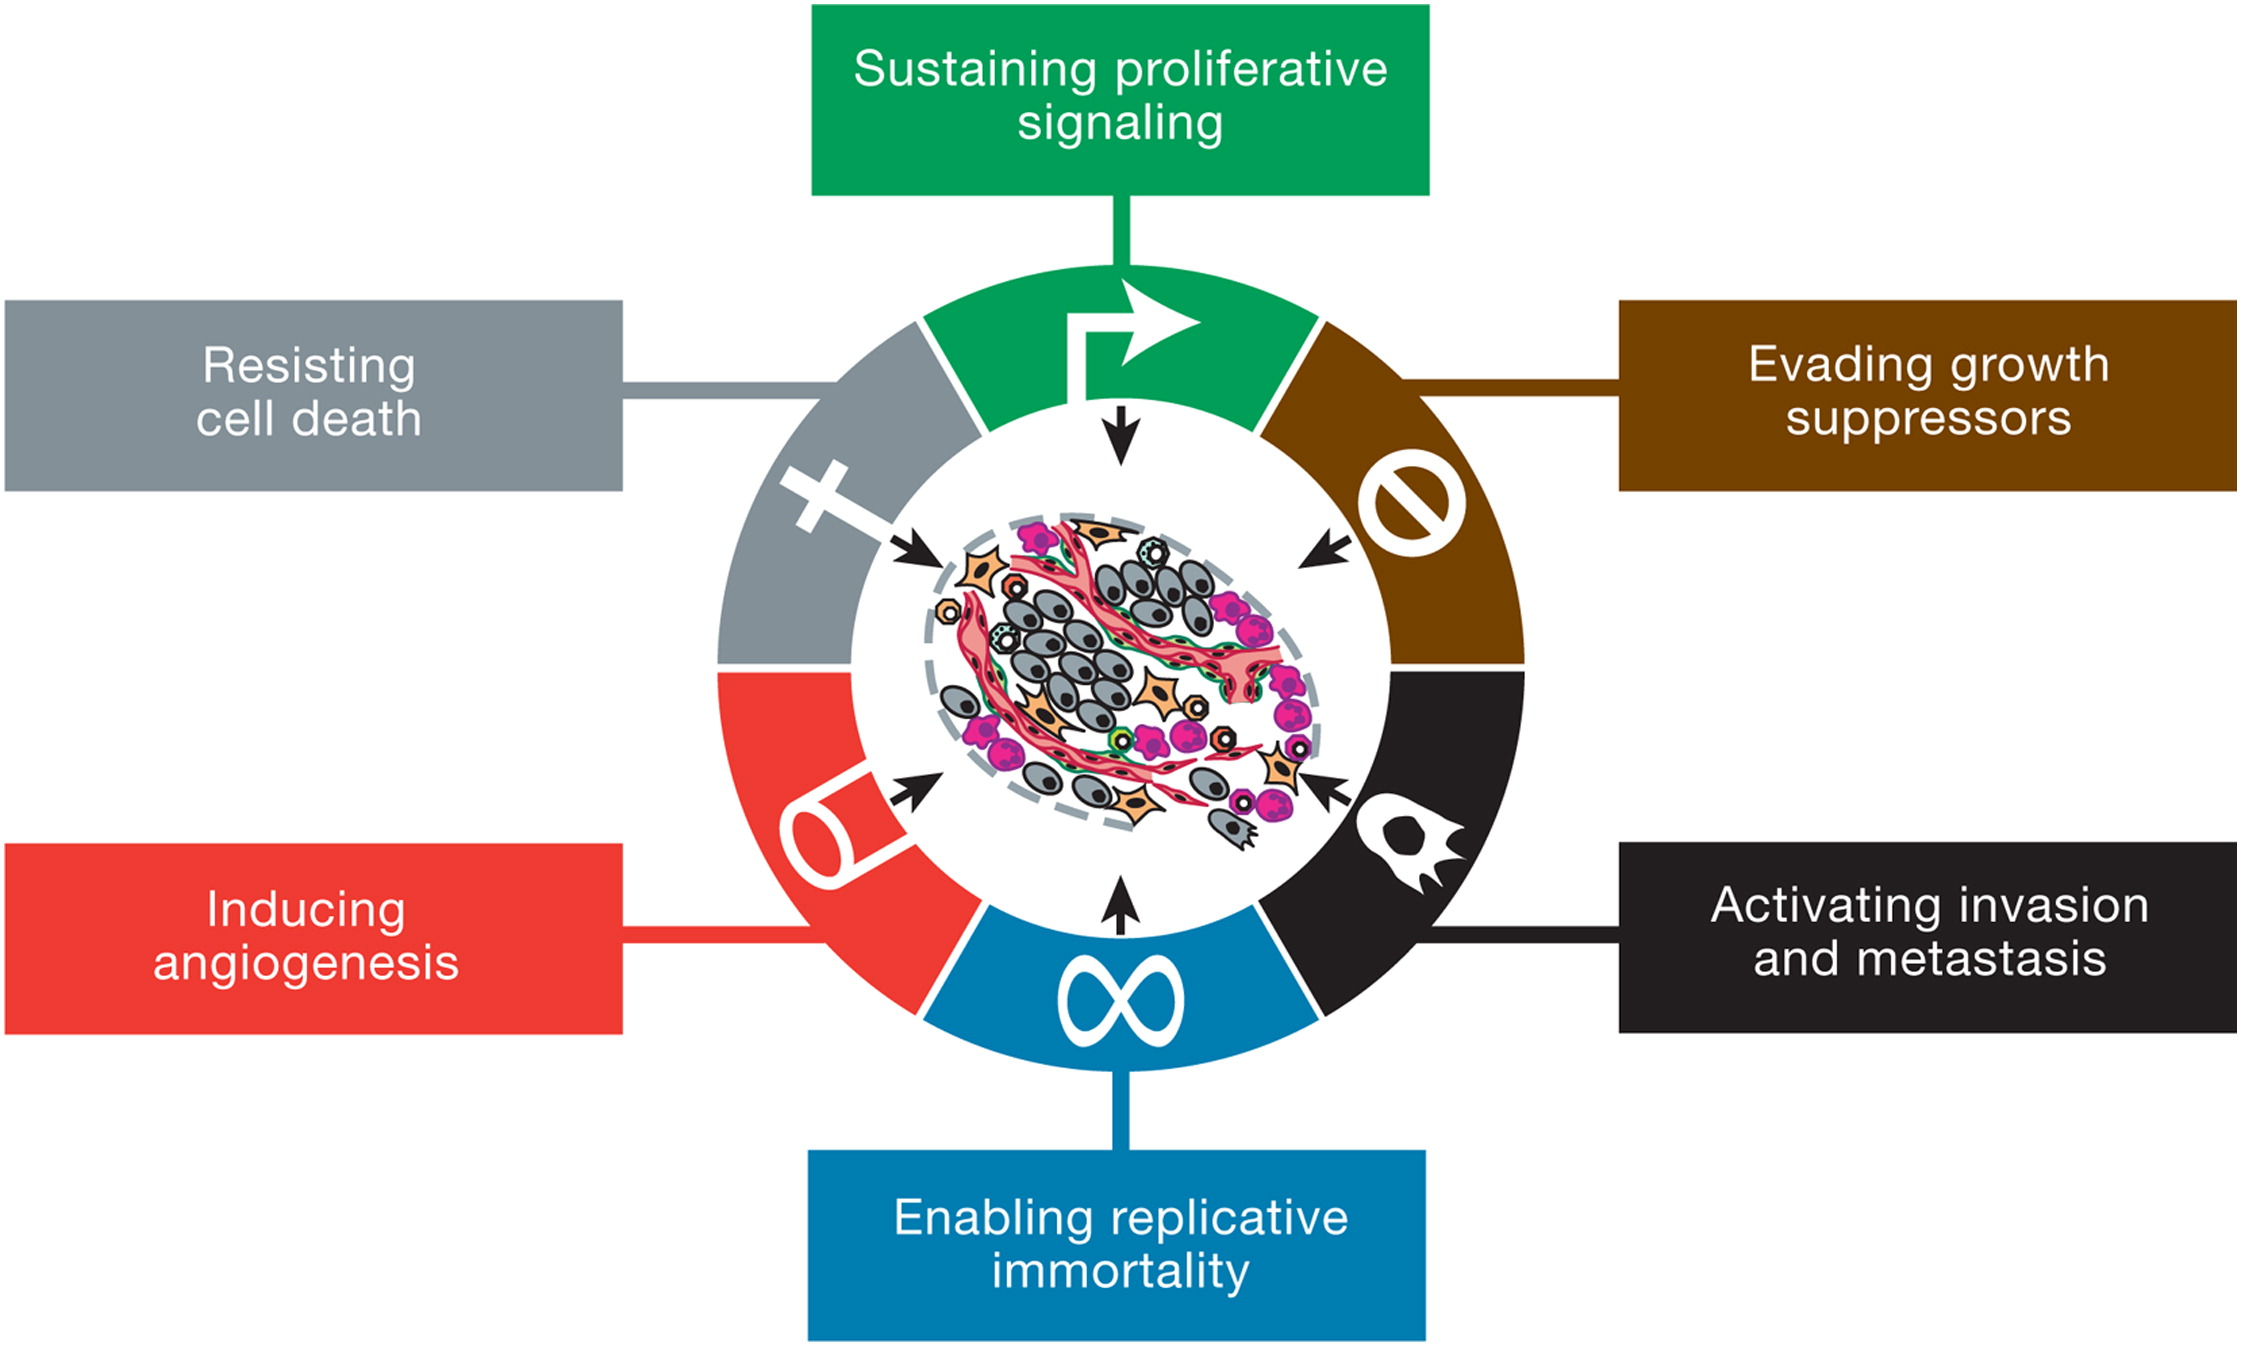
\includegraphics[width=0.8\textwidth,height=0.8\textheight,keepaspectratio]{Sections/Lit_review/Resources/tumour_causes.jpeg}
    \caption{Hallmarks for the cancer tumours\cite{Hanahan2011-px}. The Sustaining proliferative signalling feature means that the cancerous cell will be 'encouraged' to divide while evading the growth suppressors and resist cell death will only aid the birth of new malign cells. On top of that, these cells have the replicative immortality trait. Activating invasion and metastasis means that the cells are capable of spreading to other parts of the body. Lastly, angiogenesis refers to the tumours capability to draw nutrients to sustain itself through the creation of blood vessels. }
    \label{fig:hallmarks_cancer}
\end{figure}

% Small paragraph showing the ideas
Numerous sources are causing genetic alterations in a healthy organism which can lead to diseases. From \cref{fig:hallmarks_cancer} it can be seen that a large proportion of the tumour hallmarks are related to the cell division cycle that is because of all the properties of a cell, this is the one that comes under most natural selection because it leads to growth/expansion of the tumour. From evading growth suppressors to resisting cell death, the cancerous cell will not stop dividing and will slowly conquer the tissue as the healthy cells will reach the end of their cycle and die.

A driving motivation in cancer research is to learn the gene mechanisms to develop a cure for the disease. Medicine made important progress in cancer research \& diagnosis but cancer remains an unsolved problem. One of the reasons for this is the intricate mechanism of gene interactions that due to its complexity is difficult to understand. On top of that, it is not feasible to collect the ideal data\footnote{The ideal genomic dataset is represented by a large number of tumour samples, matched with a blood sample, and multi-omic sequenced (proteins, RNA, mutations etc.). Multiple samples from the same donor to track genetic changes as the disease progress and map it to the appropriated genes.)} to make accurate predictions; imagine a person suffering from cancer and scientists constantly asking for more data (i.e. biopsy). Thus, due to both ethical and clinical considerations, samples are typically taken at the point of cancer surgery, so repeat samples are usually impracticable . Therefore, it is challenging to determine the exact gene interactions which drive a subtype of cancer and as a matter of fact, any disease. 
% introducing the datasets and the efforts to get data that may be useful for us. This includes:
%  expression, mutation and signalling 
Sequencing techniques are becoming more affordable every year, and now companies like 10X Genomics can extract gene expression information at the single cell level. In addition, we get mutation data with base-pair precision; i.e. we know which part of the gene sequence presents an anomaly. Even with the costs lowering every year, sequencing large cohorts is expensive, and there are just a few large studies such as The Cancer Genome Atlas which has been used in this project.


\Cref{s:lit:bladder_cancer} introduces the reader to the bladder cancer by providing an overview of the global and local impact of the disease to both the patients and the healthcare system. It also presents the molecular characteristics of the bladder cancer and what is known at the moment of writing. The chapter then continues with an introduction of the non-cancerous dataset with the molecular properties.

\subsection{Bladder Cancer} \label{s:lit:bladder_cancer}
% Overview of the bladder cancer stats
According to Cancer Research UK, bladder cancer is the 10th most common cause of cancer and the 11th most common cancer in the UK \cite{Cancer_Research_UK2015-cf}. This is equivalent to $\sim10,000$ cases from which  $\sim5000$ are deaths, with a 5-year survival rate of 52.6\%. In 2008\cite{Ferlay2010-sx} the worldwide estimates for bladder cancer was $\sim380,000$ new cases and $\sim150,000 $deaths per year. In 2020\cite{Sung2021-hn} , there were $\sim573,000$ cases with $\sim212,536$ deaths reported which shows a considerable increase in the cancer cases\footnote{A good resource to get an overview of the prevelance of bladder cancer (and other cancers too) is the website from World Health Organisation, particularly the trends in cancer overtime: \href{https://gco.iarc.fr/en}.}. Men are 3 times more likely to develop bladder cancer and bladder cancer is specific to Western countries \cite{Knowles2015-mu}. 

% Talk about bladder cancer causes, economical burden
One of the main causes of bladder cancer is caused by smoking, being thought to provoke 50\% of the cases \citet{Knowles2015-mu}. However, the underling biological process on how smoking causes cancer is not understood. Other environment risk factors are metal contamination such as arsenic-water or exposure to ionising radiation \citet{Knowles2015-mu}. 

% Types ands stages of bladder cancer
There are multiple systems to classify bladder depending on their utility. For medical doctors there are two popular systems to dichotomies the bladder cancer Tumour-Node-Metastasis (TNM) and the Internail Sociecty of Urological Pathology (ISUP). The stages of the bladder cancer and the two naming conventions can be seen in \cref{fig:lit:bladder_cancer_stages}; image taken from the bladder cancer review from \citet{Knowles2015-mu}. The figure should be taken as an illustration of the stages and their classification, and not as the evolution of the bladder cancer.

\begin{figure}[!htb]    
    \centering
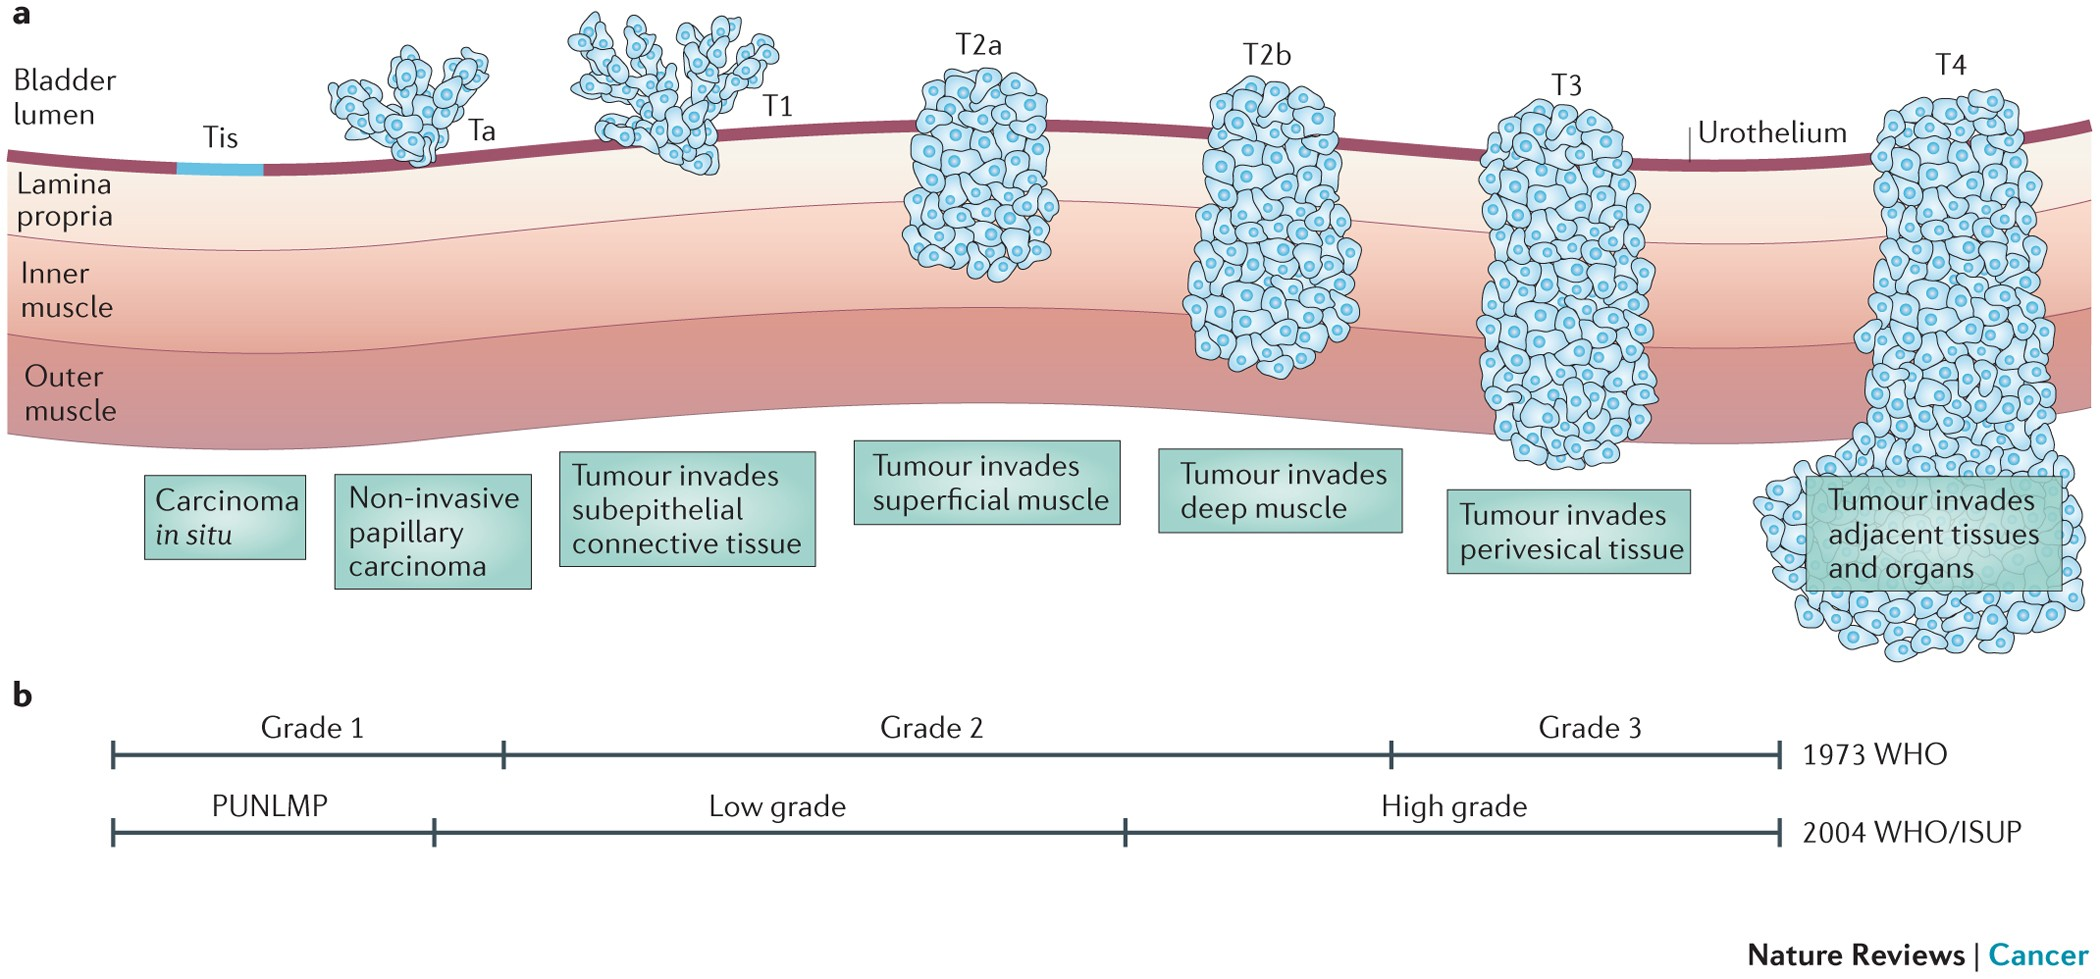
\includegraphics[width=0.9\textwidth,height=0.9\textheight,keepaspectratio]{Sections/Lit_review/Resources/bladder_cancer_grading.jpg}
    \caption{"Bladder cancer grading and staging" from \cite{Knowles2015-mu}. It displays the two grading of the bladder cancer based on its stage. Image a) should be taken just as an illustration of the different stages of bladder cancer and not mistaken with the disease evolution. }
    \label{fig:lit:bladder_cancer_stages}
\end{figure}


There are two main types of bladder cancer: non-muscle invasive (NMIBC) and muscle-invasive bladder cancer (MIBC). From \cref{fig:lit:bladder_cancer_stages} stages Tis, Ta and T1 are classified as NMIBC as they do not invaded the muscle. NMIBC appears in $\sim70\%$ of the bladder patients, it has a high 5-year survival rate with $\sim90\%$, it frequently recurs in 50-70\% of the cases and only 10-15\% progress to muscle invasion \cite{Knowles2015-mu}. Thus, patients suffering from this type of bladder cancer have favourable prognostics but their quality of life is impact as they need to attend periodical cystocopies checkups.

The muscle invasive bladder cancer encompass the T2a, T2b, T3 and T4 stages and it appears in $\sim30\%$ of the bladder cancer cases. It is more aggressive than the NMIBC with $\sim50\%$ 5-year survival prognosis, almost half of the cases of MIBC develop metastasis and for these patients the median survival is 12-15 months\cite{Knowles2015-mu}. Usually the metastatic sites for bladder cancer are lung, livers and the bones.

The patients diagnosed with MIBC undergo cystectomy which removes the entire bladder and has a larger impact to quality of life, while the NIMBC patients have regular cystocopies checkups. Both procedures have a negative impact of the patients and carer's quality of life, and bring an financial burden to them and the healthcare system. Thus, there is a need to develop better diagnosis tools and treatment plants for bladder cancer, especially for the MIBC.

\subsubsection{MIBC subtyping}

In this section there are three main studies on MIBC stratification covered, the work from TCGA \citet{Robertson2017-mg}, Lund group \cite{Marzouka2018-ge} and the MIBC consensus \cite{Kamoun2020-tj}. These three studies are particularly important for this project as TCGA is the main tumour dataset used and the consensus is the referential classification on MIBC research. The subtypes derived by the Lund group have been used to verify the results in this project against a non-TCGA based group.

There are two main parts of each of the study that are highly relevant for this project: the methods used for cluster the gene expression and the biological output. Despite the consensus work combining multiple studies, TCGA and the Lund classifications, hold their relevance by offering list of genes specific to each subtype. 

The Sankey plot in figure \cref{fig:lit:classifier_comp} shows the difference in sample classifications across the three studies covered in this project.

\begin{figure}[!htb]   
\centering
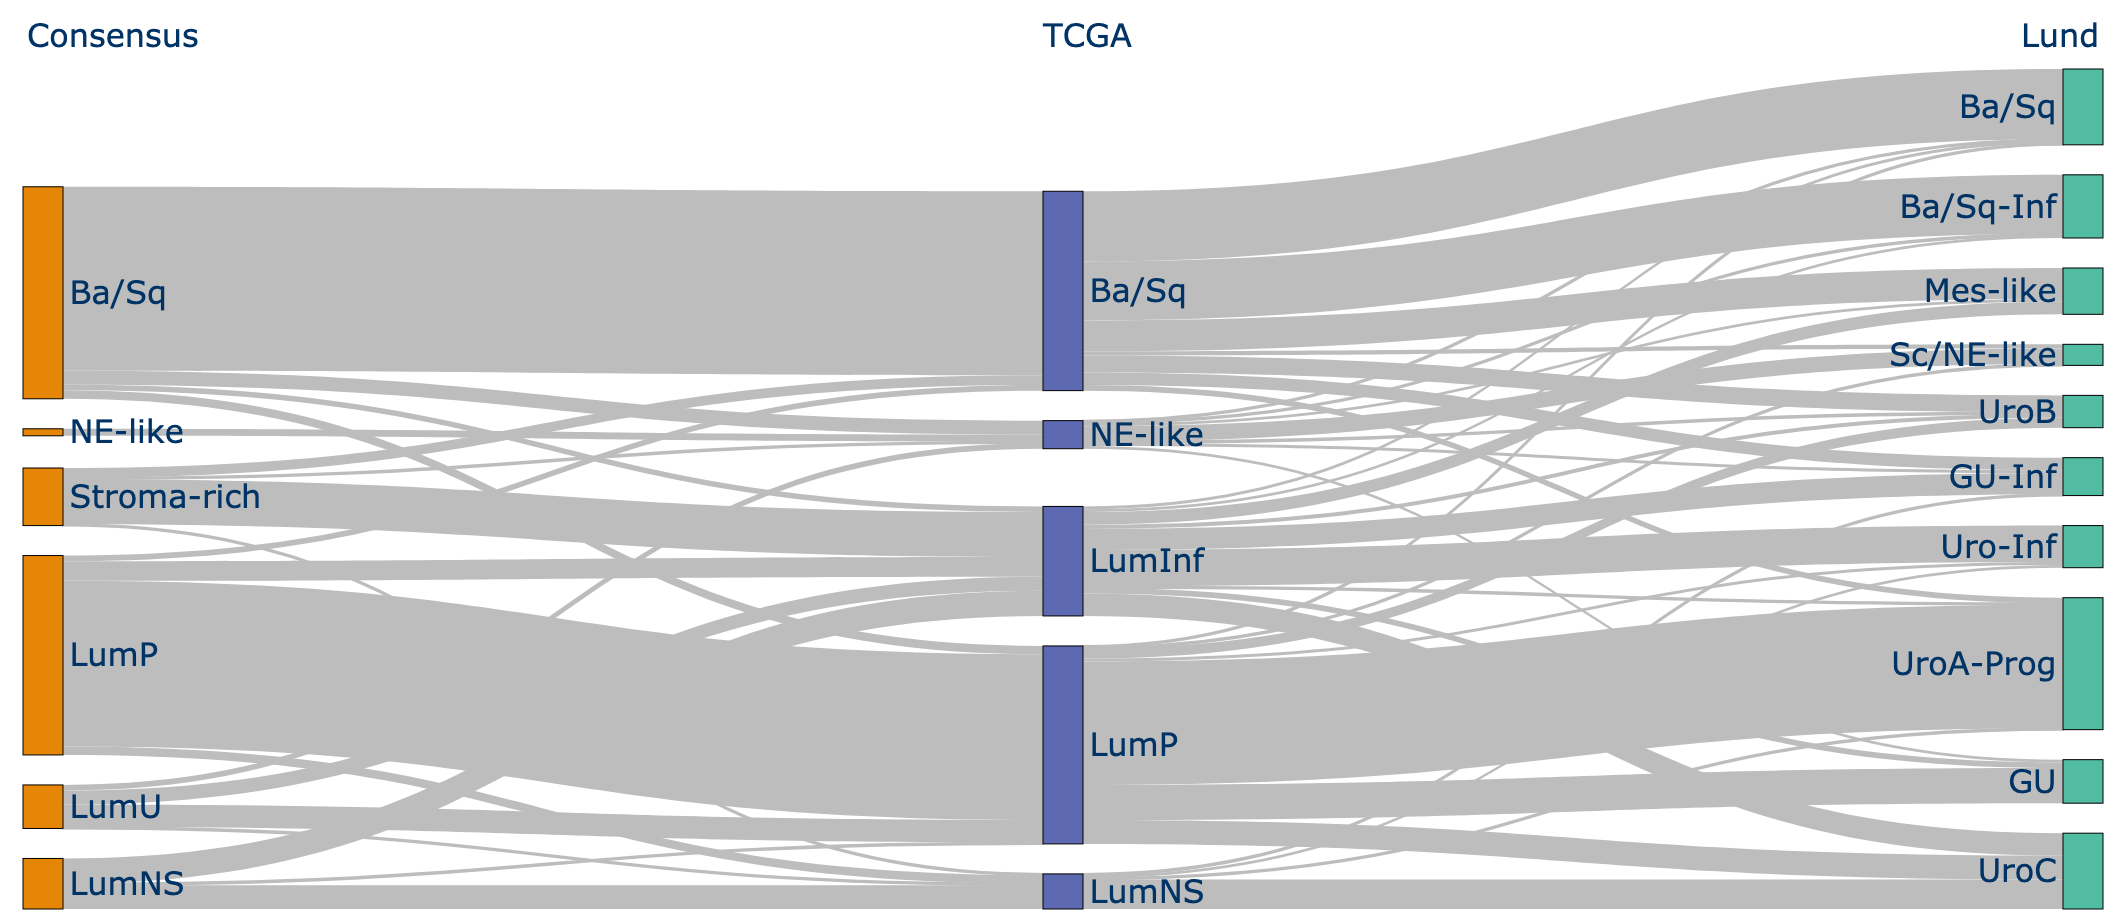
\includegraphics[width=1.0\textwidth,height=1.0\textheight,keepaspectratio]{Sections/Lit_review/Resources/classifier_differences.png}
  \caption{Showing the differences between the 3 studied classifiers}
\label{fig:lit:classifier_comp}
\end{figure}
\FloatBarrier

\paragraph*{TCGA}

% Introduction of TCGA
There are two comprehensive studies of the muscle-invasive bladder cancer (MIBC) cohort from The Cancer Genome Atlas (TCGA) \citet{Tcga2014-dr} and \citet{Robertson2017-mg}. The first is the initial research analysing the fist batch of patient samples (131) while the other analysed the entire cohort of 412 patient samples. The MIBC cohort from TCGA is an invaluable asset for the research community as a number of sequencing techniques were applied to the samples: mRNAseq (gene expression), WEX and WGS (somatic mutations), microarray-based (copy number variations) as well as metadata about the patients. This cohort is characterised by aggressive tumours, having a high grade muscle invasive and contains 408 tumour samples.

% Talk about the TCGA subtypes
In the work of \citet{Robertson2017-mg} multiple data types are analysed separately, centring on the subgroups derived from gene expression and then correlating with the other data analysis. The main result being the stratification of the MIBC into five distinct molecular subtypes: $35\%$- Luminal Papillary (LumP), $19\%$ Luminal infiltrated (LumInf), $6\%$ Luminal, $35\%$ Basal Squamous (Ba/Sq) and $5\%$ Neuronal. The highest 5-year survival is given by the Luminal subgroups while the Neuronal has the worst prognosis. 

Throughout their work \citet{Robertson2017-mg} offer a comprehensive description of the genes that are expressed in the their stratification system. The subtypes, gene specific and their function are presented in \cref{tab:lit:tcga_genes}.


\paragraph*{Lund}

% Introduce Lund cohort
At the Lund University, Sweden, there has been another effort from \citet{Sjodahl2017-xr,Marzouka2018-ge} to stratify the MIBC. The work also known as the Lund classifier, compromised 307 tumour aggressive samples on which microarray sequencing was performed to determine the gene expression. Apart from the different sequencing technology, what sets the Lund cohort apart is the immunohistochemical (IHC) matched (mostly) dataset which informed their previous stratification \citet{Sjodahl2017-xr}, only based on the gene expression,

% Clustering approach
As in the most studies on cancer stratification based on gene expression, \citet{Sjodahl2017-xr} applied a stepwise hierarchical clustering to the 307 sample finding 6 subtypes. This was then followed by the work of \citet{Marzouka2018-ge} (same lab) which used the IHC information to further split into 10 groups and create a classifier\footnote{precursor of the consensus classifier}. In the later work, the group select 1200 of the most representative genes of the classes by applying a bootstrapping-like method.

\citet{Marzouka2018-ge} applied their 10 groups classifier on the MIBC cohort from TCGA as show in \cref{fig:lit:classifier_comp}. There are four Urothelial-like subtypes UroA-Prog, Uro-Inf, UroB and UroC, two genomically unstable GU and GU-inf, two Basal/Squamous cell carcinoma (SCC) Ba/Sq and Ba/Sq-inf, and two other groups Mes-like and Small-cell/neuronendocrine (Sc/Ne). \Cref{fig:lit:lund_fig} from \citet{Marzouka2018-ge} offer a good overview of the specific gene expression to each of the Lund subtypes and \cref{tab:lit:lund_genes} is a summary of the highlighted genes for the main groups.


Compared to the other classifiers, the Lund group name the luminal samples Urothelial like and with the addition of the IHC data, the authors were able to find smaller groups which a high concentration of infiltrated cells; see \cref{fig:lit:classifier_comp} for comparison. The additional knowledge from IHC, makes the study an invaluable resource that enriches the MIBC understanding and understanding. In addition, there are several scores developed by combining multiple gene expression to help the stratification. Basal/Squamous ratio, \textit{ERBB} score or the circuit score are all used to separate the luminal from basal, GU from Uro-b or stromal from the basal, as see in \cref{fig:lit:lund_fig}.


\begin{figure}[!htb]   
\centering
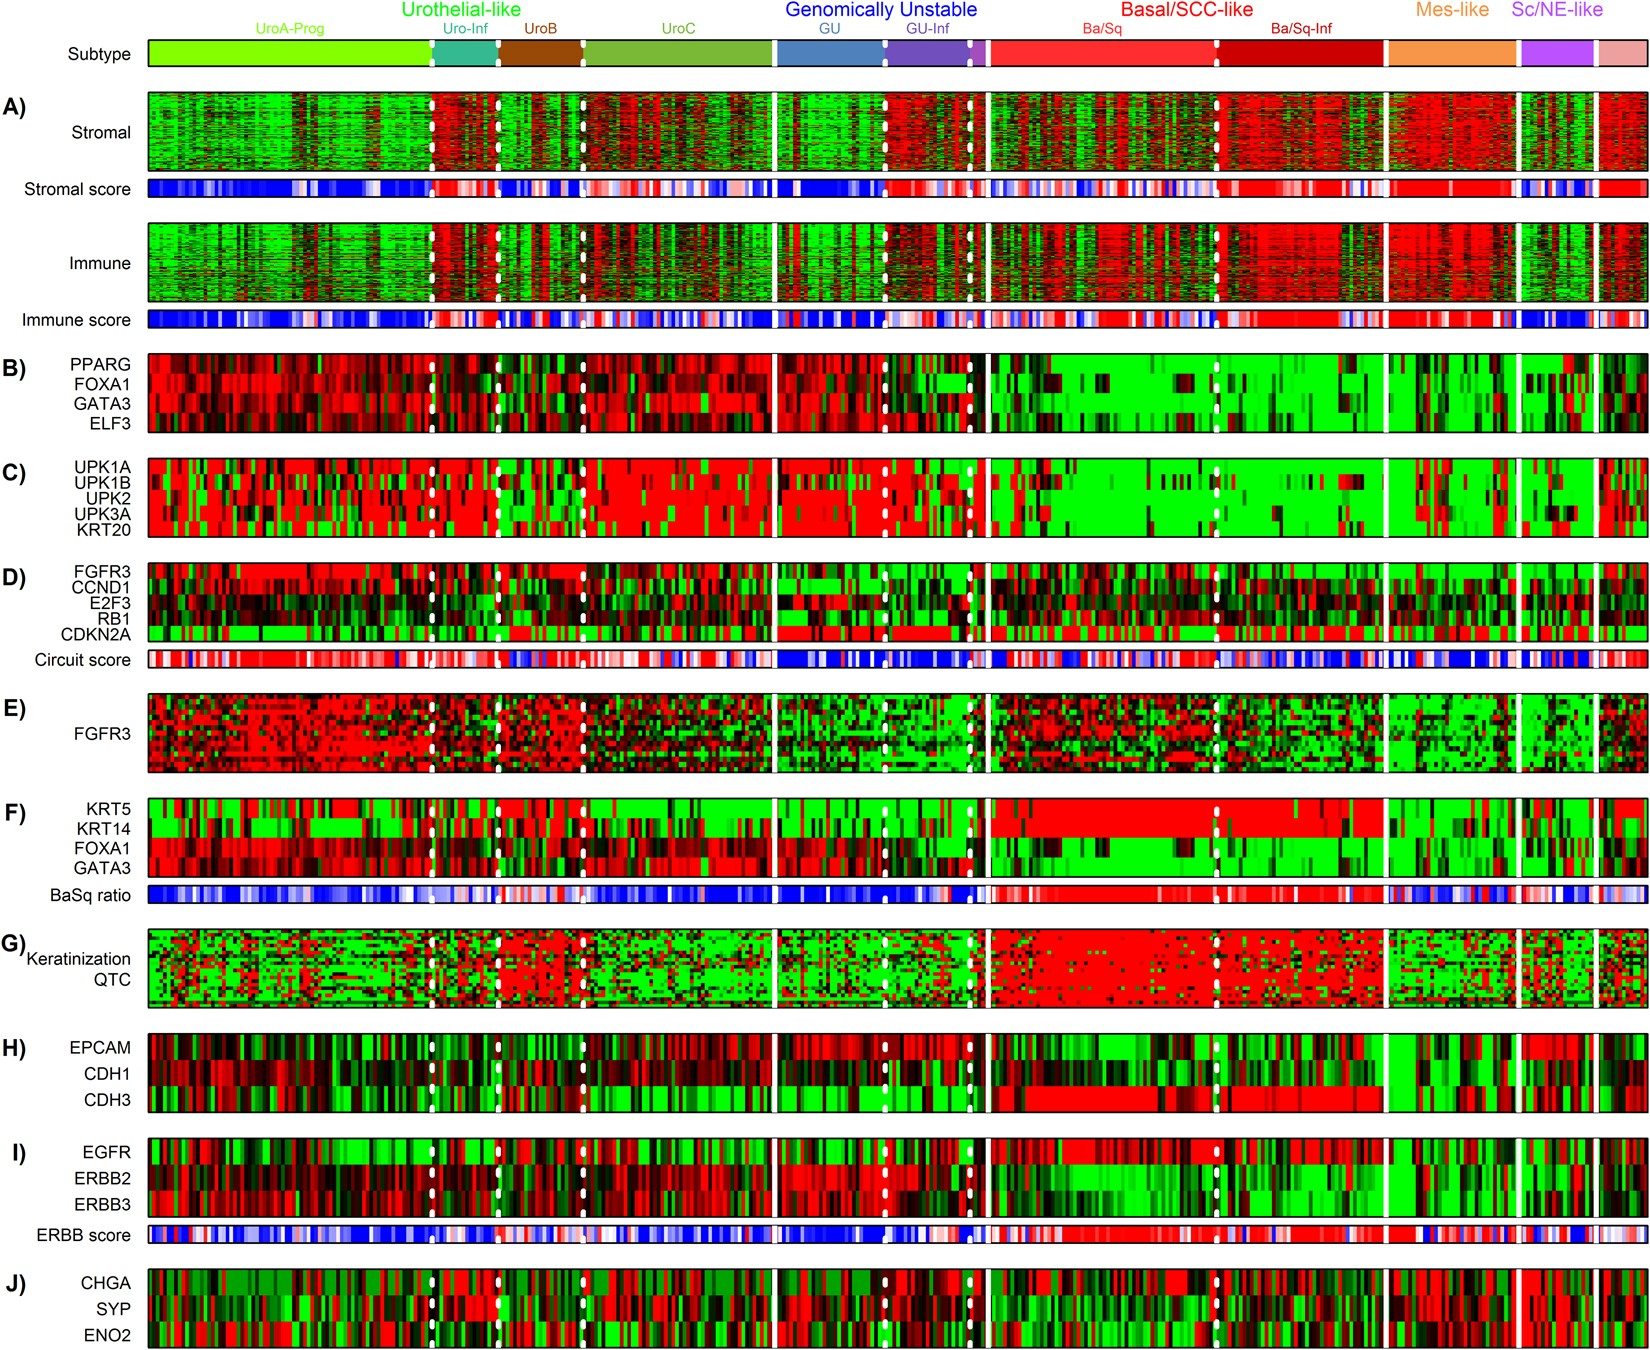
\includegraphics[width=1.0\textwidth,height=1.0\textheight,keepaspectratio]{Sections/Lit_review/Resources/Lung_subtypes.jpg}
  \caption{Subtyping the MIBC cohort from TCGA using the Lund classifier \cite{Marzouka2018-ge}. A) represents the stromal and immune cell signatures as well as the scores computed with the ESTIMATE tool\cite{Yoshihara2013-wq}. B-J represents subtype-specific signature scored as well as the Circuit, Ba/Sq ratio and \textit{ERBB} which aids the separation of subtypes. The signature scores are summarised in \cref{tab:lit:lund_genes} and image is taken from \cite{Marzouka2018-ge}.
}
\label{fig:lit:lund_fig}
\end{figure}
\FloatBarrier


\paragraph*{Consensus}

% Introducing the consensus work
The TCGA and Lund cohorts are part of the effort from \citet{Kamoun2020-tj} to find a consensus among the multiple studies on MIBC stratification. There a total of six different cohorts used in the consensus and apart from the two already mentioned \citet{Kamoun2020-tj} it also utilises the work of \citet{Mo2018-rl, Damrauer2014-tc, Choi2014-ed, Rebouissou2014-ep}. This resulted in 6 subtypes which can be seen in \cref{fig:2020_consens} with their characteristics. It can be noticed that some subtypes are more prevalent than others, with Luminal Papillary (24\%) and Basal/Squamous (35\%) being most common, followed by Luminal Unstable and Stroma Rich (both 15\%). Moreover, each subtype has a different mutations signature only enforcing the project hypothesis by adding mutation to the RNAseq data will yield better cancer classifications.

The main output of this work is an R package\footnote{See the \url{https://github.com/cit-bioinfo/consensusMIBC}.} that can classify a tissue sample based on the expression of 857 genes which were found to cover the properties of the six consensus MIBC subtypes. Initially the authors selected 857 genes that are the most representative for the six subtypes which was computed by using the statistical test LIMMA moderate t-tests\footnote{For more details check section 'Single-sample transcriptomic classifier construction' from the Supplementary document of the consensus. Alternatives approaches for classifications have been discussed by \citet{Eriksson2022-vw}}. The centroids represent the mean value of these genes across the six different datasets used. For each sample to classify, the Pearson correlation is computed and the column (i.e. consensus subtype) with the highest value represents the MIBC group; if the Pearson correlation is $<0.2$ the samples remains unclassified. 


TCGA and Lund studies offered a least of the genes specific to each subtype which were summarised in two tables \cref{tab:lit:tcga_genes} and \cref{tab:lit:lund_genes}. In contrast, the MIBC consensus does not provide a clear defined list of genes specific to each subtype, but a classification tool based on selected genes and a summary of the molecular properties as seen in \cref{tab:lit:consensus_genes}. The tool is valuable and useful for the bladder cancer research community, however one can then ask if the lack of a succinct list of genes is not an indirect consequence of the heterogeneity of the disease, and with this the challenges of studying it. 

\begin{figure}[!htb]   
\centering
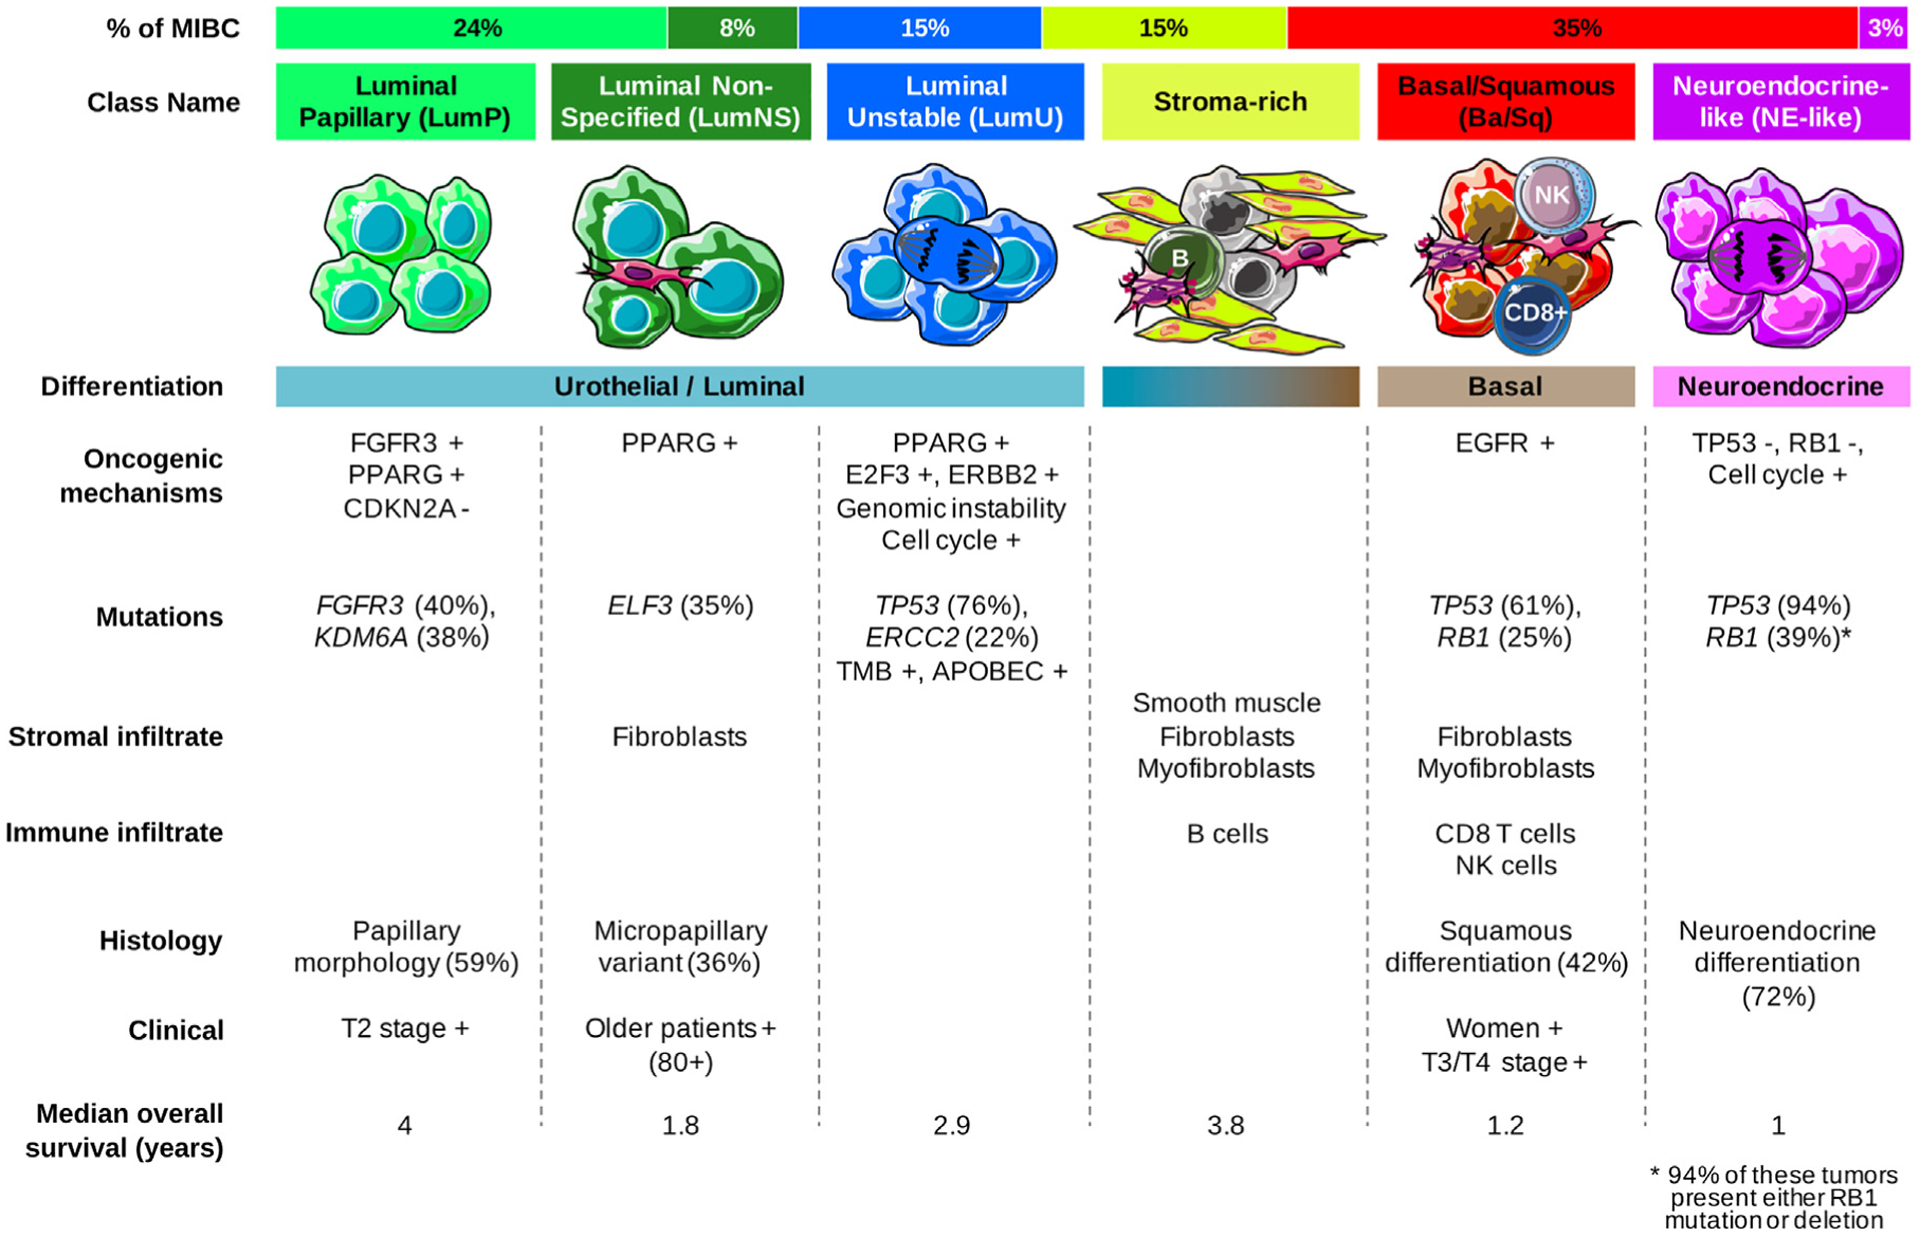
\includegraphics[width=1.0\textwidth,height=1.0\textheight,keepaspectratio]{Sections/Lit_review/Resources/2020_consensus_subtypes.jpg}
  \caption{The six different subtypes of \acrfull{mibc} by the consensus classifier\cite{Kamoun2020-tj}, the names are based on their differentiation status, morphology etc. There are three different types of Luminal Bladder cancer: most common being the ones related to papillary morphology (LumP), Luminal Non-Specified (LumNS) showing immune markers, and Luminal Unstable (LumU) is the newest luminal subtype. Basal/Squamous (Ba/Sq) is the most common bladder cancer and is related to the Squamous tissue. Neuroendocrine-like (NE-like) share similarities with Ba/Sq cancer and Stroma-rich are likely not to be a biological group but a collection of samples that contain artefacts from the collection or/and other intermediate processes. Imaged adapted from \cite{Kamoun2020-tj}.
}
\label{fig:2020_consens}
\end{figure}
\FloatBarrier


\subsubsection{Other omics}

% Some properties of the bladder cancer
% - highly mutated, a lot of epginetic changes
The research conducted by \citet{Alexandrov2013-gi} studies the mutational signatures across the human tumour types, covering $\sim7000 $cancer samples from which 20 distinct mutational signatures were extracted. \Cref{fig:lit:cancer_mut_sig} shows the mutation burden across the tumour types, with the skin cancer being the most mutated type. The bladder cancer has the 4th highest mutation burden with Signatures 13, 2 and 5 from COSMIC database\cite{Tate2019-yj}. Signature 2 and 13 are related to APOBEC family activity which are triggered by immune response. Signature 5 is unknown but it is thought to related to the mutations accumulated through ageing. 

\begin{figure}[!htb]    
    \centering
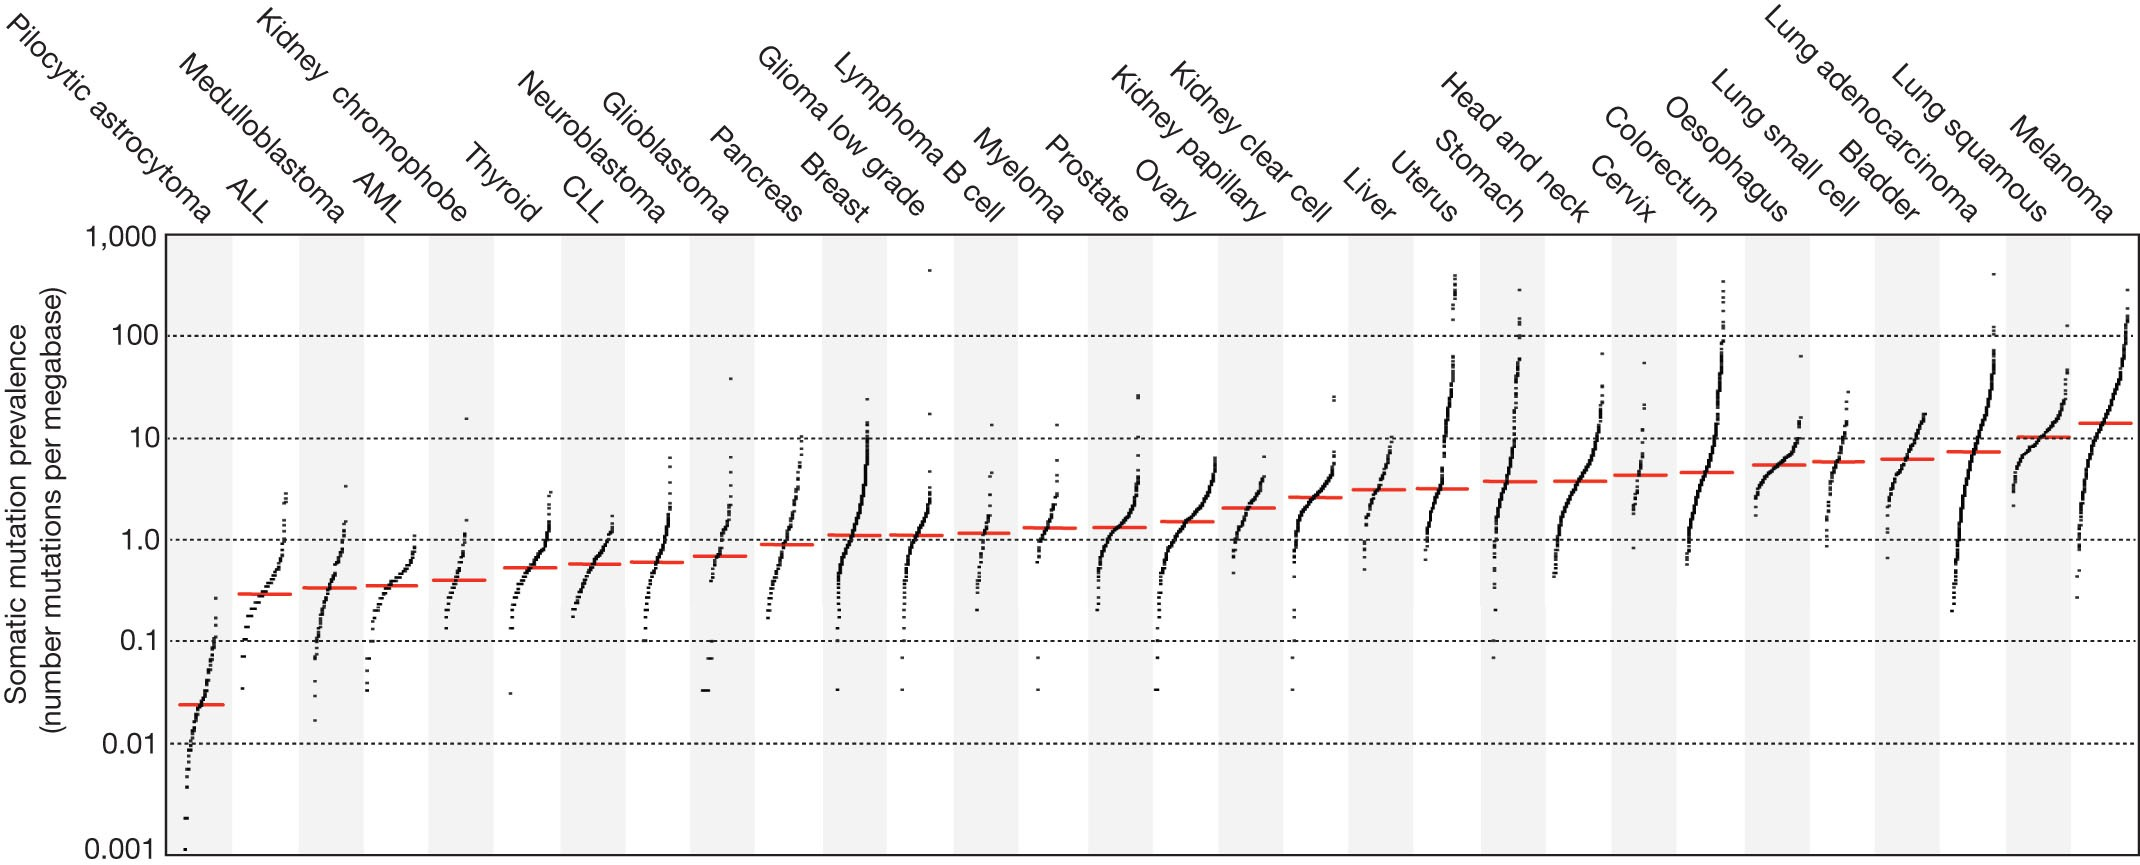
\includegraphics[width=0.9\textwidth,height=0.9\textheight,keepaspectratio]{Sections/Lit_review/Resources/mut_sig_cancers.jpg}
    \caption{Image from \cite{Alexandrov2013-gi} showing the somatic mutations across the different human cancer. Each sample is represented by a dot and the red line is the median number of mutation in that tumour type. The y-axis is the number of mutations per megabases, and the cancer types are ordered by the median mutation count, which makes bladder cancer the 4th highest mutated cancer.}
    \label{fig:lit:cancer_mut_sig}
\end{figure}

\begin{figure}[!htb]    
    \centering
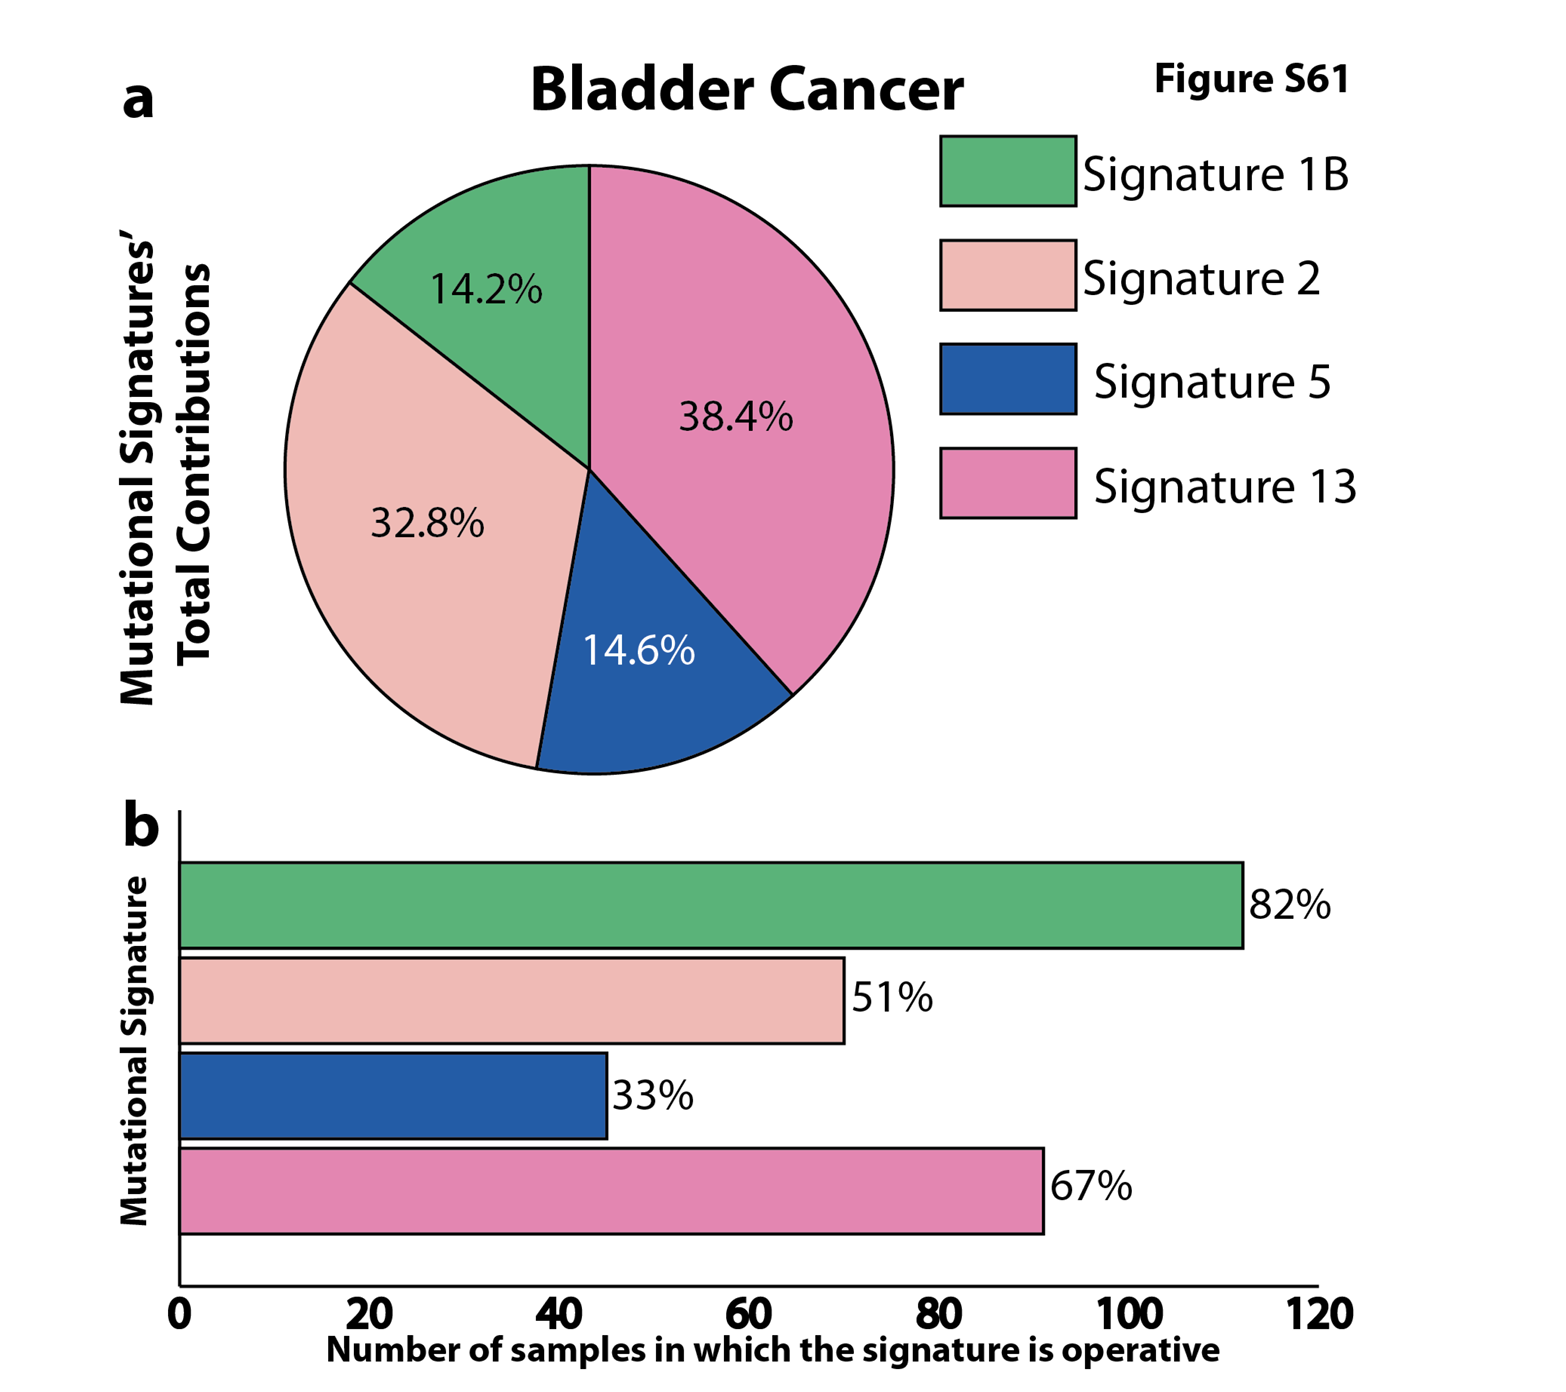
\includegraphics[width=0.6\textwidth,height=0.6\textheight,keepaspectratio]{Sections/Lit_review/Resources/bladder_mut_sig.png}
    \caption{Image from Supplementary \cite{Alexandrov2013-gi} showing the mutation signatures for bladder cancer. a) showing the the contribution of each signature while b) the number of samples where it was found. }
    \label{fig:lit:bladder_mut_sig}
\end{figure}


% epigenetic burden
The high somatic mutation burden is also highlighted by other research \cite{Tcga2014-dr, Robertson2017-mg, Kamoun2020-tj}. The first two studies found that the mutations disrupt the epigenetic machinery. Understanding these anomalies have the potential to lead to new potential targeted treatments.


\subsection{Clinical translation}


\begin{figure}[!htbp]    
    \centering
\includegraphics[width=0.9\textwidth,height=0.9\textheight,keepaspectratio]{Sections/Lit_review/Resources/robetson_summary_immune.png}
    \caption{Adapted version of Figure 1 from \cite{Robertson2023-na} showing the 82 pre-treatment samples clustered in the five discovered groups. A) Showing the response to the immune treatment split in three categories: complete response (CR), partial response (PR) and non-response (NR). S3 having the best response followed by S2 and S5. B) The recurrence rate of the MIBC in the five groups, S5, S2 and S3 showing the highest \textbf{no} recurrence rate C) How are the five groups classified by the other grouping conventions.}
    \label{fig:lit:immune_rob}
\end{figure}


The MIBC heterogeneity and the challenging aspect of finding clinical relevant subgroups is also shown in the subsequent work \citet{Robertson2023-na} from the lead author in the TCGA study \cite{Robertson2017-mg}. The more recent study concentrates on a smaller cohort of 82 patients that underwent pembrolizumab treatment\footnote{This is a type of immunotherapy offered to patients with advanced MIBC and metastatic,} with the goal to understand the molecular profiles of the aggressive tumours that did not respond to traditional treatments. The pre-treatment tumour samples were clustered in five different subtypes each with different recurrence rate as seen in \cref{fig:lit:immune_rob}. S3, S2 and S5 exhibited the highest response (A) to the treatment which also had the best \textbf{no} recurrence rate (B). \Cref{fig:lit:immune_rob} (C) shows how the five groups in \cite{Robertson2023-na} are classified by the other classifications (TCGA \cite{Robertson2017-mg}, Consensus \cite{Kamoun2020-tj}, Lund \cite{Marzouka2018-ge} and MD Aderson \cite{Dadhania2016-cb}). Even though \citet{Robertson2023-na} found statistical significance similarities between the immune therapy response groups and the other classification, the five new subtypes exhibit new properties and were not clear situated on the previous groups; as seen in \cref{fig:lit:immune_rob} (C), particularly S3 or S4 subgroups which are not easily identifiable with one of the previous subtypes.

At the moment of writing the thesis (mid 2024), there is an ongoing clinical trial, GUSTO (Gene expression subtypes of Urothelial carcinoma: Stratified Treatment and Oncological outcomes), which uses the TCGA subtypes to determine the treatment for patients suffering of aggressive bladder cancer. The study is based in the UK, it will consist of 320 patients over 3 years, and are using a commercially available called Decipher Bladder\footnote{See \url{https://www.veracyte.com/decipher-bladder/}} but using the TCGA classification and not company's subgrouping\cite{Griffin2024-zr}. The patients will be randomised, some will receive the standard treatment while the others the treatment specific to their disease subtype. There are three different plans for Basal\&Neuronal, Luminal infiltrated, and Luminal Papillary \& Luminal.

The above two translational clinical efforts highlight the weight of the TCGA study from \citet{Robertson2017-mg} in bladder classification. Especially that the GUSTO trial has used the TCGA classifier over the consensus or even Lund cohort which had the IHC information. It also underlines the importance of a good classifier and the importance of having well-define clusters. For example, the LumInf TCGA subtype has its own immunotherapy treatments in the GUSTO trial \citet{Griffin2024-zr} but there is a large variance between the consensus, TCGA and Lund classifiers as seen in \cref{fig:clustering_types}. This is a strong motivator for the project and for combining multiple data types at the computational level.


\subsection{Datasets used}

There are two important types of datasets used in this project: the data on non-cancerous bladder from Jack Birch Unit (JBU) and MIBC cohort from The Cancer Genome Atlas (TCGA). The first helps build a representation of the urothelium which is as close as possible to the healthy tissue which is then use to inform the tumour stratification.

The TCGA datasets are central for this project, contributing with the gene expression from RNAsequencing and the somatic mutations from Whole Exome Sequencing (WES). In addition to this, the metadata available is used to compute the different survival rates for the subtypes derived. 

At the moment of writing (mid 2024), the TCGA dataset is publicly available from the Genomics Data Central (GDC) portal\footnote{A new user needs to set an agreement with the GDC in order to have access \url{https://portal.gdc.cancer.gov/}}, while the JBU data on non-cancerous is in the process on getting published and hosted on a portal.

As taking a bladder biopsy is an invasive procedure it is not possible to take samples from healthy patients, thus benign disease were used to form a non-cancerous molecular representation of the bladder. These samples included overactive bladder (OAB), stress urinary incontinence (SUI), non-visible haematuria (NVH), post-prolapse staging, survey after a tension-free vaginal tape (TVT) procedure, and other less normal conditions such as cystitis cystica (CC) and a patient suffering with recurrent UTI (rUTI).

The non-cancerous dataset from JBU compromised 88 samples from which 49 are Abs-Ca differentiated (Diff), 23 P0 and 14 Undifferentiated (UD). The first type of samples are specialised tissue grown in-vitro, developing barrier function (like the bladder) following the Abs-Ca protocol from \cite{Cross2005-fe}. The P0 biopsies were sequenced immediately before doing anything lab work on the tissue. The UD data are processed P0 following \cite{Cross2005-fe} to an undifferentiated state. 

The Abs-Ca samples were grow in the lab to exhibit the 'purer' markers of the urothelium differentiation and molecular properties of the healthy bladder tissue. The P0 samples exhibit the differentiation markers as in the Diff biopsies but it will contain some other cells infiltration, thus making the bladder molecular signal is less clear. By their nature both Abs-Ca and P0 will be closer to Luminal samples in the MIBC. The UD are on the other side of the differentiation spectrum and are closer to Basal MIBC subtypes. Thus, the non-cancerous dataset it has an imbalanced built in, having a higher representation of the differentiated tissue. 

To both dataset the Kallisto method was used to align the RNA-seq reads using genome version GRCh38 with Gencode annotation version 42 which resulted in $\sim33k$ genes for each dataset.


\subsection{Summary}


\pagebreak

\subsection{Tables}


% TCGA table
\begin{table}[htbp]
\centering
\caption{The molecular characterisation of the TCGA subgroups taken from the \textit{mRNA Expression-Based Molecular Subtypes} and \textit{Discussion} section Figure 2 from \citet{Robertson2017-mg}}
    \begin{tabularx}{\textwidth}{
      >{\hsize=.6\hsize\raggedright\arraybackslash}X
      >{\hsize=.8\hsize\raggedright\arraybackslash}X
      >{\hsize=.6\hsize\arraybackslash}X
    }
    \toprule
    Subtype & Genes & Description \\
    \midrule
    Luminal-papillary (35\%) & \textit{KRT20, PPARG, FOXA1, GATA3, SNX31, UPK1A, UPK2, FGFR3} & 
    \begin{itemize}[leftmargin=*, nosep, after=\vspace{-\baselineskip}, before=\vspace{-.6\baselineskip}]
        \item Characterised by \textit{FGFR3} mutations
        \item Papillary histology
        \item Low risk of progression
    \end{itemize} \\
    \midrule
    Luminal-infiltrated (19\%) & \textit{CD274, PDCD1LG2, IDO1, CXCL11, L1CAM, SAA1} & 
    \begin{itemize}[leftmargin=*, nosep, after=\vspace{-\baselineskip}, before=\vspace{-.6\baselineskip}]
        \item Lowest purity
        \item High expression of \textit{EMT} and myofibroblast markers, and of the miR-200s (tumour suppressor)
        \item Medium expression of \textit{CD274, CTLA4} immune markers
        \item May respond to immune checkpoint therapy
        \item May be resistant to cisplatin-based chemotherapy
    \end{itemize} \\
    \midrule
    Luminal (6\%) & \textit{KRT20, PPARG, FOXA1, GATA3, SNX31, UPK1A, UPK2, FGFR3} & 
    \begin{itemize}[leftmargin=*, nosep, after=\vspace{-\baselineskip}, before=\vspace{-.6\baselineskip}]
        \item New subtype in TCGA
    \end{itemize} \\
    \midrule
    Basal-squamous (35\%) &\textit{ CD44, KRT6A, KRT5, KRT14, COL17A1}; Squamous: \textit{DSC3, GSDMC, TCGM1, PI3, TP63} & 
    \begin{itemize}[leftmargin=*, nosep, after=\vspace{-\baselineskip}, before=\vspace{-.6\baselineskip}]
        \item High incidence in women
        \item Squamous differentiation
        \item Basal keratin expression
        \item High expression of \textit{CD274, CTLA4} immune markers
        \item Might be useful for immune checkpoint therapy
    \end{itemize} \\
    \midrule
    Neuronal (5\%) &\textit{ MSI1, PLEKHG4B, GNG4, PEG10, RND2, APLP1, SOX2, TUBB2B} & 
    \begin{itemize}[leftmargin=*, nosep, after=\vspace{-\baselineskip}, before=\vspace{-.6\baselineskip}]
        \item Expression of neuroendocrine, neuronal gene and high cell-cycle signature of proliferative state
        \item The most aggressive tumours with the lowest survival rate
    \end{itemize} \\
    \bottomrule
    \end{tabularx}
    \label{tab:lit:tcga_genes}
\end{table}

% Lund table
\begin{table}[htbp]
\centering
\caption{Summary table of the work done for Lund stratification which is primarily based on the Figure 2 from \citet{Marzouka2018-ge} but it also contains some additional information from research group's earlier work from  \citet{Sjodahl2017-xr}. The suffix '-inf' represents the infiltrated nature of the subtype.}
    \begin{tabularx}{\textwidth}{>{\hsize=.6\hsize\raggedright\arraybackslash}X >{\hsize=\hsize\arraybackslash}X}
    \toprule
    Subtype & Description \\
    \midrule
    UroA and GU & 
    \begin{itemize}[leftmargin=*, nosep, after=\vspace{-\baselineskip}]
        \item The UroA and GU tumours exhibit two signatures known in urothelial cell differentiation 1) \textit{PPARG, FOXA1, GATA3, ELF3} and 2) \textit{UPK1A, UPK1B, UPK2, UPK3A, KRT20}. These are the genes also seen in the Luminal subtypes form TCGA (\textbf{check this}).
        \item The difference between GU and Uro subtypes is given by the up/down-regulated of \textit{FGFR3, CCND1, E2F3, RB1, CDKN2A}.
    \end{itemize} \\
    \midrule
    Basal/Squamous & 
    \begin{itemize}[leftmargin=*, nosep, after=\vspace{-\baselineskip}]
        \item The signatures of \textit{KRT5, KRT14, FOXA1 and GATA3} are definitory for the Basal/Squamous tumours (Ba/Sq). 
        \item Keratinization signature: \textit{KRT5, KRT6A, KRT6B, KRT6C, KRT14, KRT16}
        \item Cell adhesion genes \textit{EPCAM, CDH1, CDH3} differentiate the Basal tumours from the squamous.
        \item The Basal/Squamous are also separated from the Uro and GU subtypes by the difference in expression of the tyrosine kinase receptors \textit{EGFR, ERBB2, ERBB3}.
    \end{itemize} \\
    \midrule
    MES-like & 
    \begin{itemize}[leftmargin=*, nosep, after=\vspace{-\baselineskip}]
        \item Similar to Sc/NE-like, but are less infiltrated
    \end{itemize} \\
    \midrule
    Sc/NE-like & 
    \begin{itemize}[leftmargin=*, nosep, after=\vspace{-\baselineskip}]
        \item As in the case for Basal, high in \textit{KRT5, KRT14}, low in \textit{FOXA1, GATA3}
        \item High expression in\textit{ CHGA, SYP, ENO2}
        \item More infiltrated than the MES-like
    \end{itemize} \\
    \bottomrule
    \end{tabularx}
    \label{tab:lit:lund_genes}
\end{table}

% Consensus table
\begin{table}[htbp]
\centering
\caption{The molecular characterisation of the MIBC subgroups taken based on the consensus work of \cite{Kamoun2020-tj}. It summaries sections\ textit{ 3.2 and 3.3 } from the main paper. LumP, LumNS and LumU exhibit more differentiation status characteristics and contain \textit{PARG/GATA3/FOXA1}-related Lund signature.}
    \begin{tabularx}{\textwidth}{>{\hsize=.8\hsize\raggedright\arraybackslash}X >{\hsize=\hsize\arraybackslash}X}
    \toprule
    Subtype & Description \\
    \midrule
    Luminal-papillary (LumP) (24\%) & 
    \begin{itemize}[leftmargin=*, nosep, after=\vspace{-\baselineskip}]
        \item High expression of noninvasive Ta pathway signature
        \item Mutations in \textit{FGFR3, KDM6A}
    \end{itemize} \\
    \midrule
    Luminal non-specified (LumNS) (8\%) & 
    \begin{itemize}[leftmargin=*, nosep, after=\vspace{-\baselineskip}]
        \item Elevated stromal infiltration signatures
        \item \textit{ELF3} mutations, activated by \textit{PPARG//RARG}
    \end{itemize} \\
    \midrule
    Luminal unstable (LumU) (15\%) & 
    \begin{itemize}[leftmargin=*, nosep, after=\vspace{-\baselineskip}]
        \item Higher cell activity compared to other luminal tumours
        \item Mutations in \textit{ERCC2, TP53}
    \end{itemize} \\
    \midrule
    Stroma-rich (15\%) & 
    \begin{itemize}[leftmargin=*, nosep, after=\vspace{-\baselineskip}]
        \item Intermediate levels of urothelial differentiation and stromal infiltration
        \item Overexpression of smooth muscle, endothelial, fibroblast and myofibroblast gene signatures
        \item Immune infiltration of T and B-cell
    \end{itemize} \\
    \midrule
    Basal/Squamous (35\%) & 
    \begin{itemize}[leftmargin=*, nosep, after=\vspace{-\baselineskip}]
        \item Mutations in \textit{KDM6A, RB1}
        \item Signatures associated with Basal
        \item Immune infiltration: cytotoxic lymphocytes, natural killer cells
    \end{itemize} \\
    \midrule
    Neuronal (3\%) & 
    \begin{itemize}[leftmargin=*, nosep, after=\vspace{-\baselineskip}]
        \item Mutations in \textit{KDM6A, RB1}
        \item Signatures associated with Basal
    \end{itemize} \\
    \bottomrule
    \end{tabularx}
    \label{tab:lit:consensus_genes}
\end{table}

